\documentclass[a4paper]{article}

\input{style/ch_xelatex.tex}
\input{style/scala.tex}

\lstset{numbers=left,
basicstyle=\tiny,
numberstyle=\tiny,
keywordstyle=\color{blue!70},
commentstyle=\color{red!50!green!50!blue!50},
frame=single, rulesepcolor=\color{red!20!green!20!blue!20},
escapeinside=\`\`
}

\graphicspath{{fig/}{fig/generated/}}
\usepackage[fontset=none]{ctex}
\usepackage{graphicx}
\usepackage{color,framed}
\usepackage{listings}
\usepackage{caption}
\usepackage{amssymb}
\usepackage{enumerate}
\usepackage{xcolor}
\usepackage{bm}
\usepackage{lastpage}
\usepackage{fancyhdr}
\usepackage{tabularx}
\usepackage{geometry}
\usepackage{minted}
\usepackage{graphics}
\usepackage{subfigure}
\usepackage{float}
\usepackage{pdfpages}
\usepackage{pgfplots}
\pgfplotsset{width=10cm,compat=1.9}
\usepackage{multirow}
\usepackage{footnote}
\usepackage{booktabs}
\usepackage{hyperref}

\setCJKmainfont{PingFang SC}
\setCJKsansfont{Heiti SC}
\setCJKmonofont{PingFang SC}
\setCJKfamilyfont{zhkai}{PingFang SC}
\newcommand{\kaishu}{\CJKfamily{zhkai}}

\geometry{a4paper,left=2.3cm,right=2.3cm,top=2.7cm,bottom=2.7cm}
\pagestyle{fancy}
\lhead{\kaishu \leftmark}
\rhead{\kaishu 深度学习及应用（高阶课）实验报告}
\lfoot{}
\cfoot{\thepage}
\rfoot{}
\renewcommand{\headrulewidth}{0.1pt}
\renewcommand{\footrulewidth}{0pt}
\setlength{\textfloatsep}{8mm}

\begin{document}
\renewcommand{\contentsname}{目\ 录}
\renewcommand{\refname}{参考文献}
\renewcommand{\figurename}{图}
\renewcommand{\tablename}{表}
\renewcommand{\today}{\number\year 年 \number\month 月 \number\day 日}

\begin{titlepage}
    \begin{center}
    
\includegraphics[width=0.8\textwidth]{NKU.png}\\[1cm]
    \vspace{20mm}
        \textbf{\huge\textbf{\kaishu{计算机学院}}}\\[0.5cm]
        \textbf{\huge{\kaishu{深度学习及应用（高阶课）实验报告}}}\\[2.3cm]
        \textbf{\Huge\textbf{\kaishu{现代卷积神经网络}}}

        \vspace{\fill}

    \centering
    \textsc{\LARGE \kaishu{姓名\ :\ 林晖鹏}}\\[0.5cm]
    \textsc{\LARGE \kaishu{学号\ :\ 2312966}}\\[0.5cm]
    \textsc{\LARGE \kaishu{专业\ :\ 计算机科学与技术}}\\[0.5cm]

    \vfill
    {\Large \today}
    \end{center}
\end{titlepage}

\renewcommand{\thefigure}{\thesection{}.\arabic{figure}}
\cfoot{\thepage\ of \pageref{LastPage}}

\clearpage
\tableofcontents
\newpage

\section{实验目的}
\begin{enumerate}
    \item 掌握卷积神经网络的基本原理与实现流程。
    \item 学会使用 PyTorch 搭建简单 CNN 完成 CIFAR-10 图像分类。
    \item 学会实现并比较 ResNet、DenseNet、MobileNet 在 CIFAR-10 上的分类效果。
    \item 扩展实现 Res2Net，并分析其相对其他卷积网络的优势与劣势。
\end{enumerate}

\section{实验设置}
% \subsection{实验环境}
% \begin{itemize}
%     \item 编程语言：Python
%     \item 深度学习框架：PyTorch、torchvision
%     \item 数据集：CIFAR-10
%     \item 训练平台：请填写本地设备或服务器配置
% \end{itemize}

% \subsection{统一实验设置}
本实验统一采用 SGD 优化器，考虑到不同模型对学习率的要求可能不同，为了减小调参压力以及尽可能公平对比，这里对学习率集合 $\{0.2, 0.1, 0.05, 0.02, 0.01, 0.005\}$ 进行搜索，批大小固定为 512，训练轮数固定为 100。各模型均以验证集最佳准确率对应的学习率作为最终配置，并记录测试集准确率、参数量、FLOPs、训练时间与推理时间等指标。

\section{模型结构设计}
\subsection{原始 CNN}
原始 CNN 由老师提供，用于作为无跳跃连接卷积网络的基础对照模型。其特点是结构简单、参数量小，但深层特征表达能力有限。

\subsection{ResNet}
ResNet 通过残差连接缓解深层网络训练中的退化问题\cite{resnet}。本文实现的是适配 CIFAR-10 的 ResNet20，使用三组残差块，通道数分别为 16、32、64。由于训练参数和训练方式多模型要统一，与原文中的批次和学习率阶梯式调整方案不一样，只能接近原文结果。

\subsection{DenseNet}
DenseNet 采用密集连接方式，使得每一层都能够复用前面所有层的特征\cite{densenet}。本文实现的是论文版本中的 DenseNet-BC-100，包含 bottleneck 和 compression 机制，修改了stem的大小。

\subsection{MobileNet}
MobileNet 采用深度可分离卷积，将标准卷积分解为 depthwise 卷积和 pointwise 卷积，从而显著降低计算量和参数规模\cite{mobilenet}。本文实现的是论文中 CIFAR-10 适配版的 MobileNetV1。

\subsection{Res2Net（扩展）}
Res2Net 在残差块内部进一步构造多尺度特征表示，使单个残差块内部也具备更细粒度的尺度建模能力\cite{Res2Net}。本文实现的是基于 CIFAR 风格骨架的 Res2Net 变体，主干由三个 stage 组成，每个 stage 含 3 个 Bottle2neck 模块，输出通道依次扩展到 256、512 和 1024，用于扩展分析。由于原论文中说明了CIFAR-10数据集上的实现以ResXNet29\_8c64w为base，但是这个宽度和通道数太大了，在bs为512情况下显存不够，这里减少这两个参数分别为4和16，经实验验证，正确率尚能接受，但是可能比完全版低，这里只是提供学习模型思路参考。

\subsection{网络结构打印结果}
按照要求，模型结构可通过 \texttt{print(net)} 直接打印。下面的内容依据当前代码重新实例化五个模型后导出，完整原始输出保存在 \texttt{model\_prints/*.txt} 中。考虑到报告总页数限制，正文中仅保留五个模型的顶层 \texttt{print(net)} 输出骨架，重复子模块以省略号表示。

\begin{table*}[htbp]
\centering
\caption{Top-level \texttt{print(net)} outputs of five models}
\scriptsize
\setlength{\tabcolsep}{4pt}
\begin{tabular}{p{0.13\textwidth} p{0.81\textwidth}}
\toprule
Model & \ttfamily print(net) excerpt \\
\midrule
CNN &
\parbox[t]{0.81\textwidth}{\ttfamily
SimpleCNN(\\
\quad (features): Sequential(Conv2d(3,32) $\rightarrow$ ReLU $\rightarrow$ MaxPool,\\
\qquad Conv2d(32,64) $\rightarrow$ ReLU $\rightarrow$ MaxPool,\\
\qquad Conv2d(64,128) $\rightarrow$ ReLU $\rightarrow$ AdaptiveAvgPool2d)\\
\quad (classifier): Sequential(Flatten $\rightarrow$ Linear(128,128) $\rightarrow$ ReLU $\rightarrow$ Linear(128,10))\\
)}
\\[2mm]
ResNet20 &
\parbox[t]{0.81\textwidth}{\ttfamily
ResNet(\\
\quad (stem): Sequential(Conv2d(3,16) $\rightarrow$ BatchNorm2d(16) $\rightarrow$ ReLU)\\
\quad (layer1): Sequential(3 $\times$ BasicBlock, channels=16)\\
\quad (layer2): Sequential(3 $\times$ BasicBlock, channels=32, first stride=2)\\
\quad (layer3): Sequential(3 $\times$ BasicBlock, channels=64, first stride=2)\\
\quad (avgpool): AdaptiveAvgPool2d((1,1))\\
\quad (fc): Linear(64,10)\\
)}
\\[2mm]
DenseNet-BC-100 &
\parbox[t]{0.81\textwidth}{\ttfamily
DenseNet(\\
\quad (stem): Conv2d(3,24,kernel\_size=3,padding=1,bias=False)\\
\quad (blocks): ModuleList(3 $\times$ DenseBlock, each block has 16 DenseLayer)\\
\quad (transitions): ModuleList(2 $\times$ TransitionLayer, compression=0.5)\\
\quad (norm): BatchNorm2d(258)\\
\quad (relu): ReLU(inplace=True)\\
\quad (avgpool): AdaptiveAvgPool2d((1,1))\\
\quad (fc): Linear(258,10)\\
)}
\\[2mm]
MobileNetV1 &
\parbox[t]{0.81\textwidth}{\ttfamily
MobileNetV1(\\
\quad (stem): Sequential(Conv2d(3,32) $\rightarrow$ BatchNorm2d(32) $\rightarrow$ ReLU)\\
\quad (features): Sequential(11 $\times$ DepthwiseSeparableConv,\\
\qquad channels 32 $\rightarrow$ 64 $\rightarrow$ 128 $\rightarrow$ 128 $\rightarrow$ 256 $\rightarrow$ 256 $\rightarrow$ 512 $\rightarrow \cdots \rightarrow$ 512)\\
\quad (avgpool): AdaptiveAvgPool2d((1,1))\\
\quad (fc): Linear(512,10)\\
)}
\\[2mm]
Res2Net &
\parbox[t]{0.81\textwidth}{\ttfamily
Res2Net(\\
\quad (stem): Sequential(Conv2d(3,64) $\rightarrow$ BatchNorm2d(64) $\rightarrow$ ReLU)\\
\quad (layer1): Sequential(3 $\times$ Bottle2neck, base\_channels=64)\\
\quad (layer2): Sequential(3 $\times$ Bottle2neck, base\_channels=128, first stride=2)\\
\quad (layer3): Sequential(3 $\times$ Bottle2neck, base\_channels=256, first stride=2)\\
\quad (avgpool): AdaptiveAvgPool2d((1,1))\\
\quad (fc): Linear(1024,10)\\
)}
\\
\bottomrule
\end{tabular}
\label{tab:model_prints}
\end{table*}

\section{实验结果分析}
\subsection{学习率搜索结果}
\begin{table*}[htbp]
\centering
\caption{Best configurations selected from learning-rate sweep}
\begin{tabular}{lccc}
\toprule
Model & Best LR & Best Val Acc & Test Acc \\
\midrule
CNN & 0.1 & 81.06\% & 76.58\% \\
ResNet20 & 0.05 & 87.14\% & 82.40\% \\
DenseNet-BC-100 & 0.2 & 87.62\% & 85.13\% \\
MobileNetV1 & 0.05 & 87.28\% & \textbf{85.64\%} \\
Res2Net & 0.05 & \textbf{89.52\%} & 85.34\% \\
\bottomrule
\end{tabular}
\label{tab:best_lr}
\end{table*}

由表中可以看出，不同模型在相同优化器下的最优学习率并不一致。

\subsection{模型综合性能对比}
\begin{table*}[htbp]
\centering
\caption{Performance comparison of each model under its best learning rate}
\begin{tabular}{lcccc}
\toprule
Model & Params & FLOPs & Train Time / s & Infer Time / ms \\
\midrule
CNN & \textbf{111,050} & \textbf{10,409,472} & \textbf{243.6} & \textbf{0.017} \\
ResNet20 & 272,474 & 41,403,072 & 781.3 & 0.054 \\
DenseNet-BC-100 & 769,162 & 300,797,106 & 2921.7 & 0.262 \\
MobileNetV1 & 1,618,250 & 41,195,008 & 775.9 & 0.054 \\
Res2Net & 3,461,834 & 913,271,808 & 3389.6 & 0.259 \\
\bottomrule
\end{tabular}
\label{tab:model_compare}
\end{table*}

综合结果表明，Res2Net 在验证集上取得了最高的最佳准确率，但其参数量、FLOPs 和训练时间也明显高于其他模型。MobileNetV1 在保持较高精度的同时具备较好的效率表现；DenseNet-BC-100 的参数量适中，但训练耗时较长；原始 CNN 虽然轻量，但分类性能最弱。

\subsection{各模型训练曲线}
\begin{figure}[H]
    \centering
    \subfigure[Train loss]{
        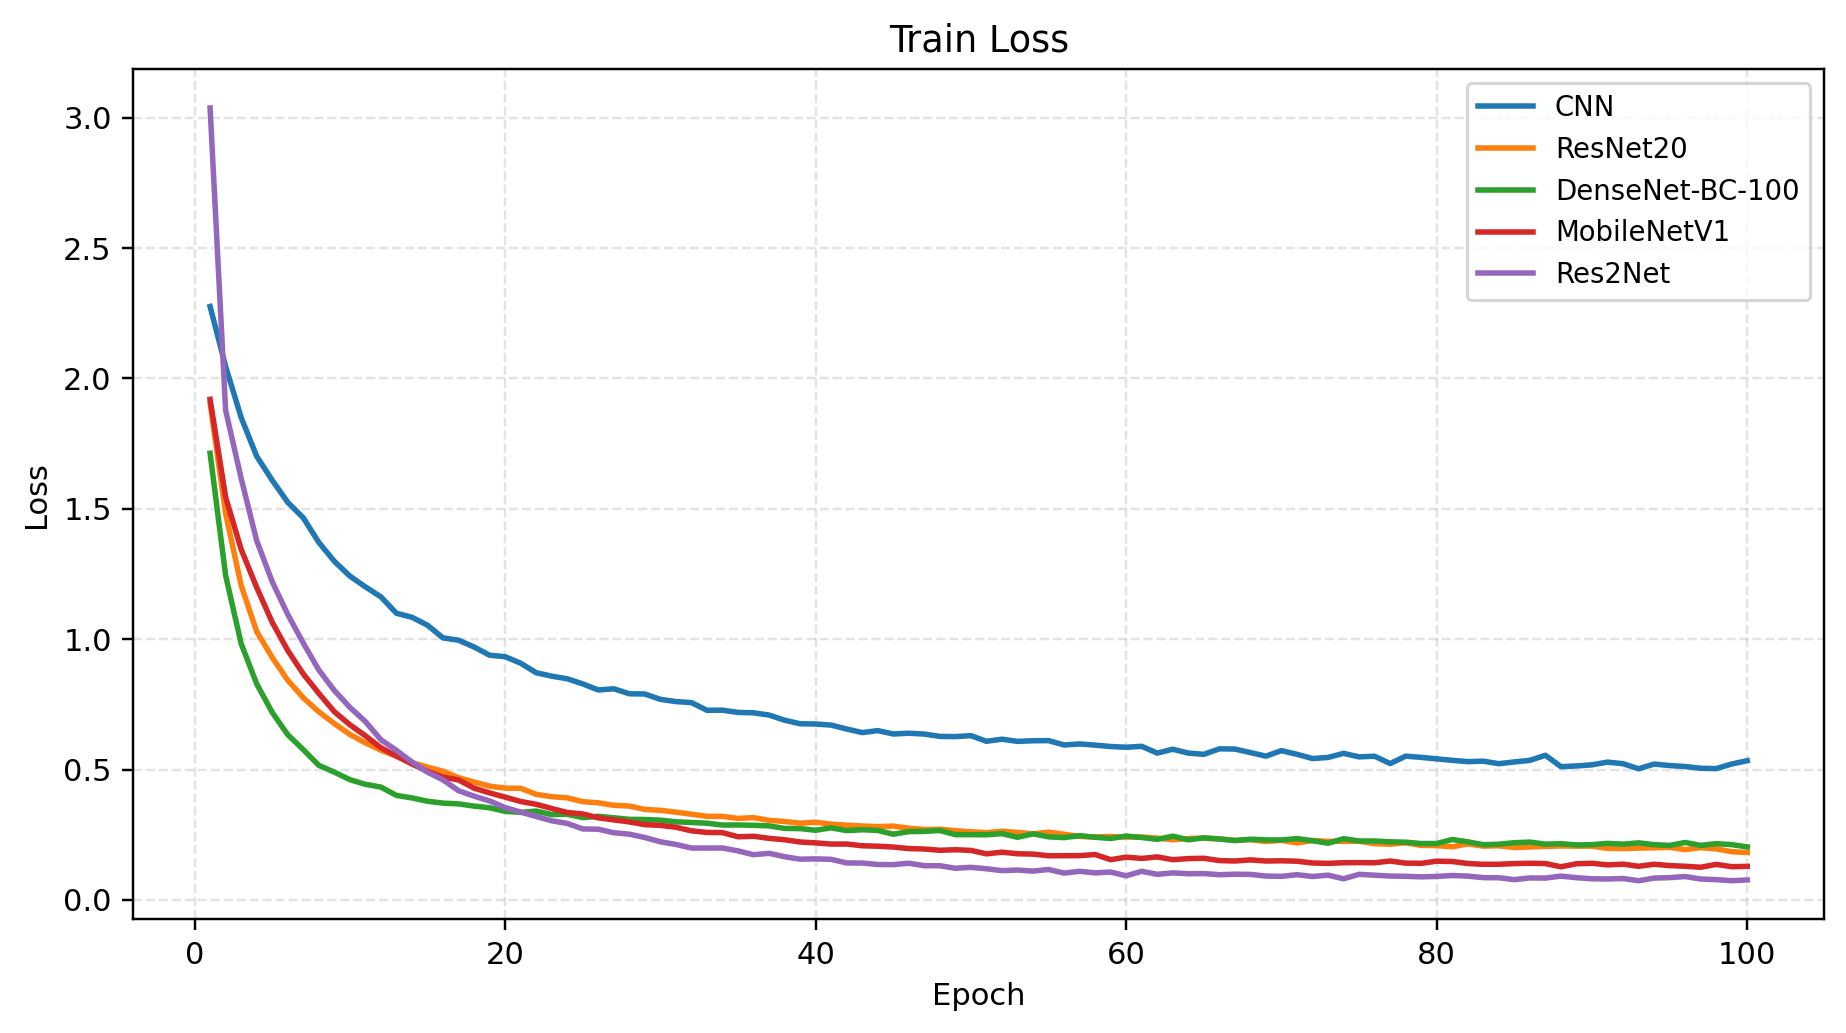
\includegraphics[width=0.47\textwidth]{generated/all_models_train_loss.png}
    }
    \subfigure[Train accuracy]{
        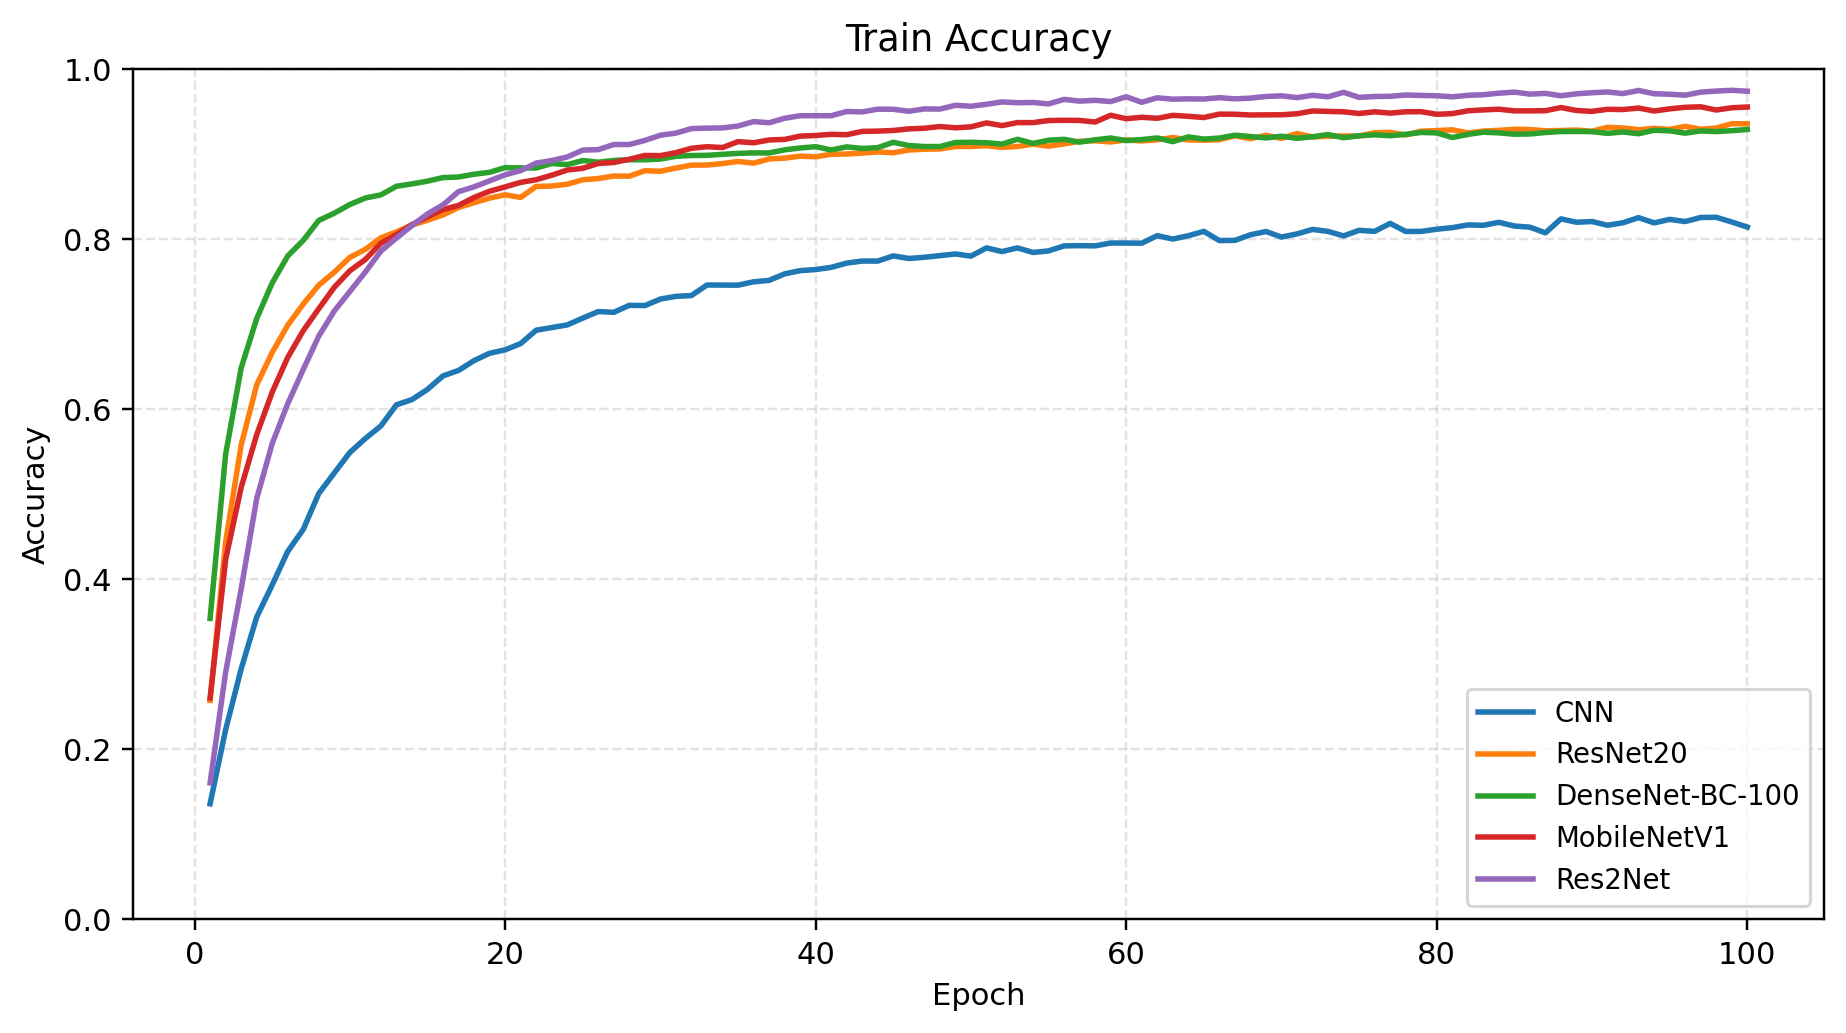
\includegraphics[width=0.47\textwidth]{generated/all_models_train_acc.png}
    }

    \subfigure[Validation loss]{
        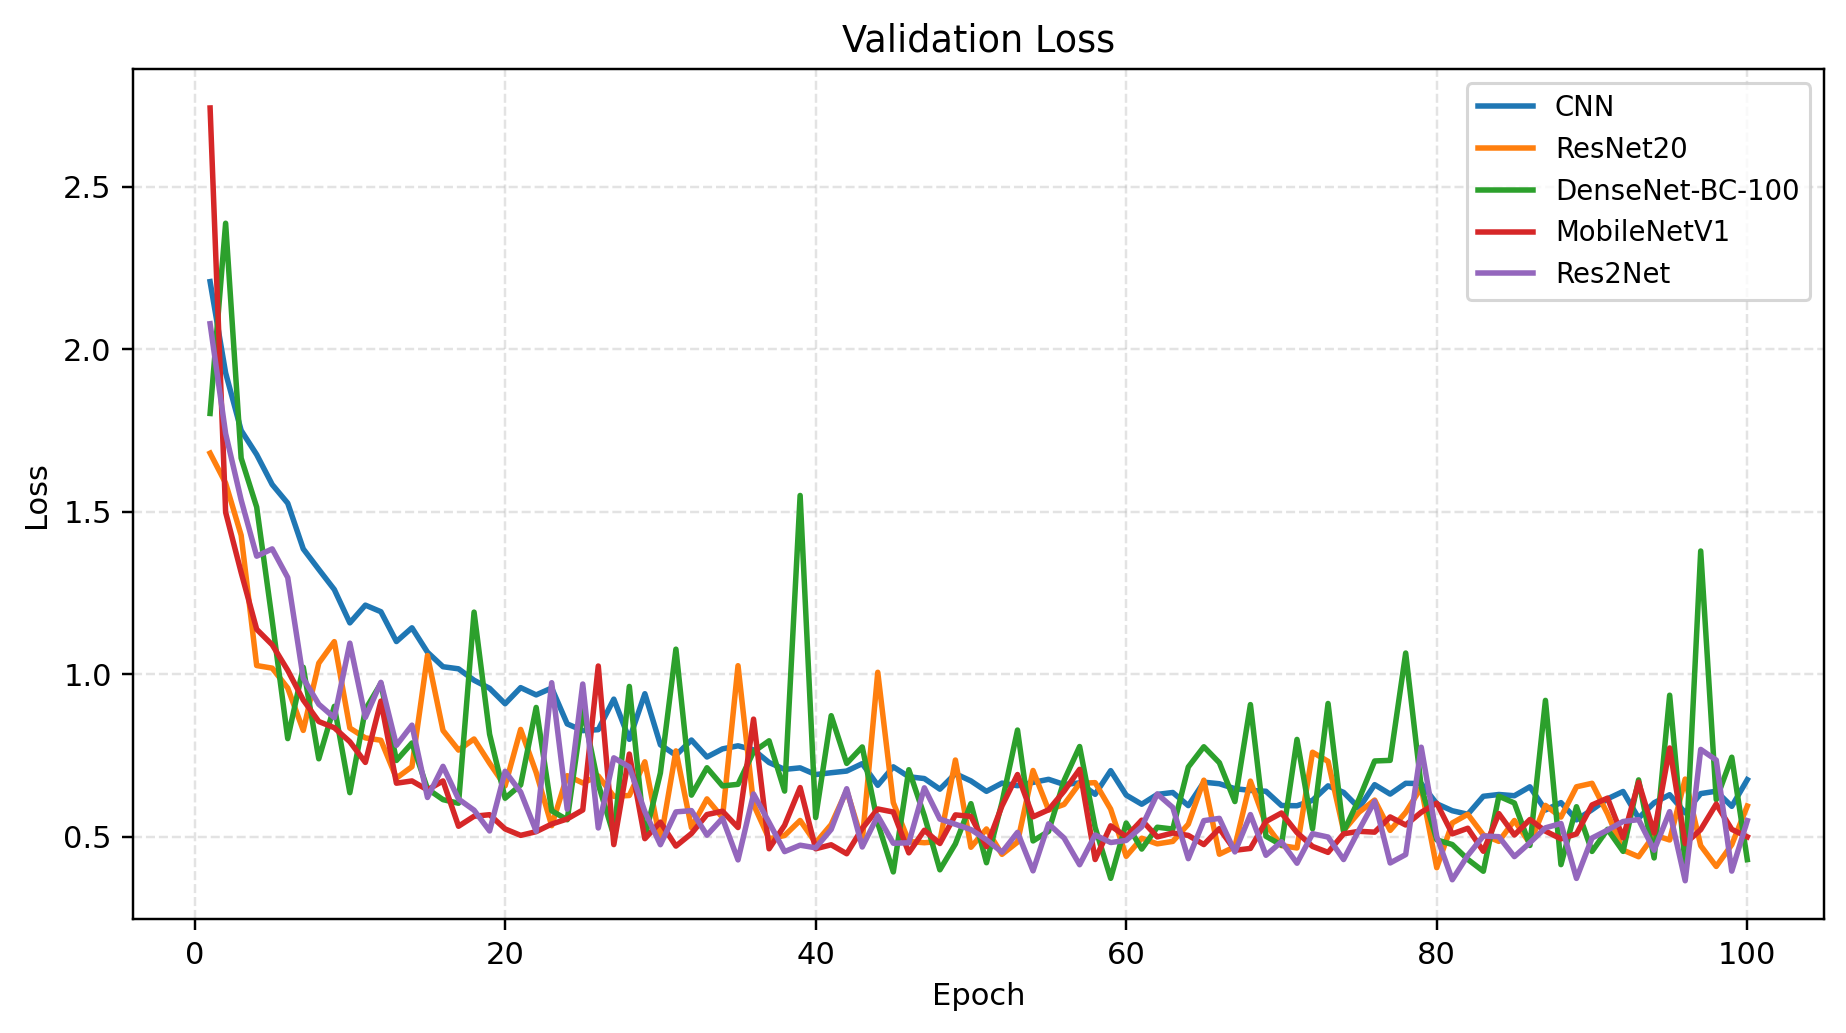
\includegraphics[width=0.47\textwidth]{generated/all_models_val_loss.png}
    }
    \subfigure[Validation accuracy]{
        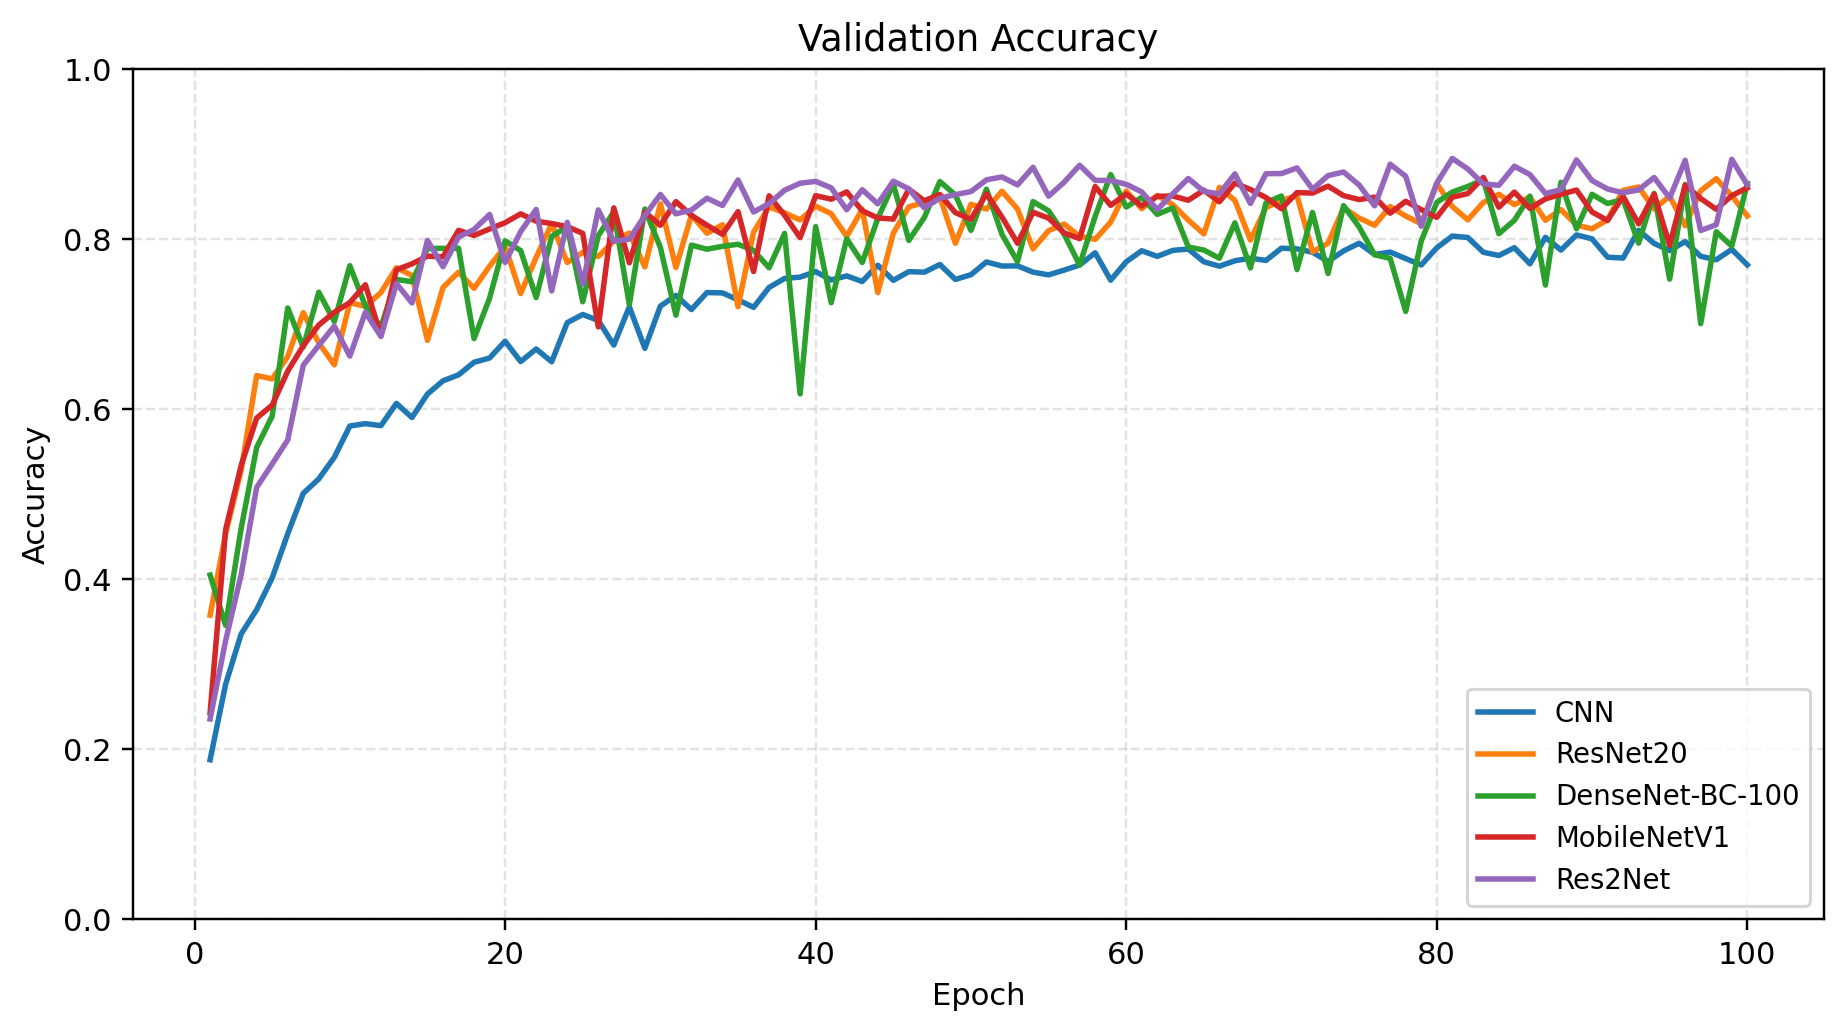
\includegraphics[width=0.47\textwidth]{generated/all_models_val_acc.png}
    }
    \caption{五种模型在最优学习率下的训练与验证曲线对比。}
\end{figure}

\subsection{类别准确率分析}
\begin{figure}[htpb]
    \centering
    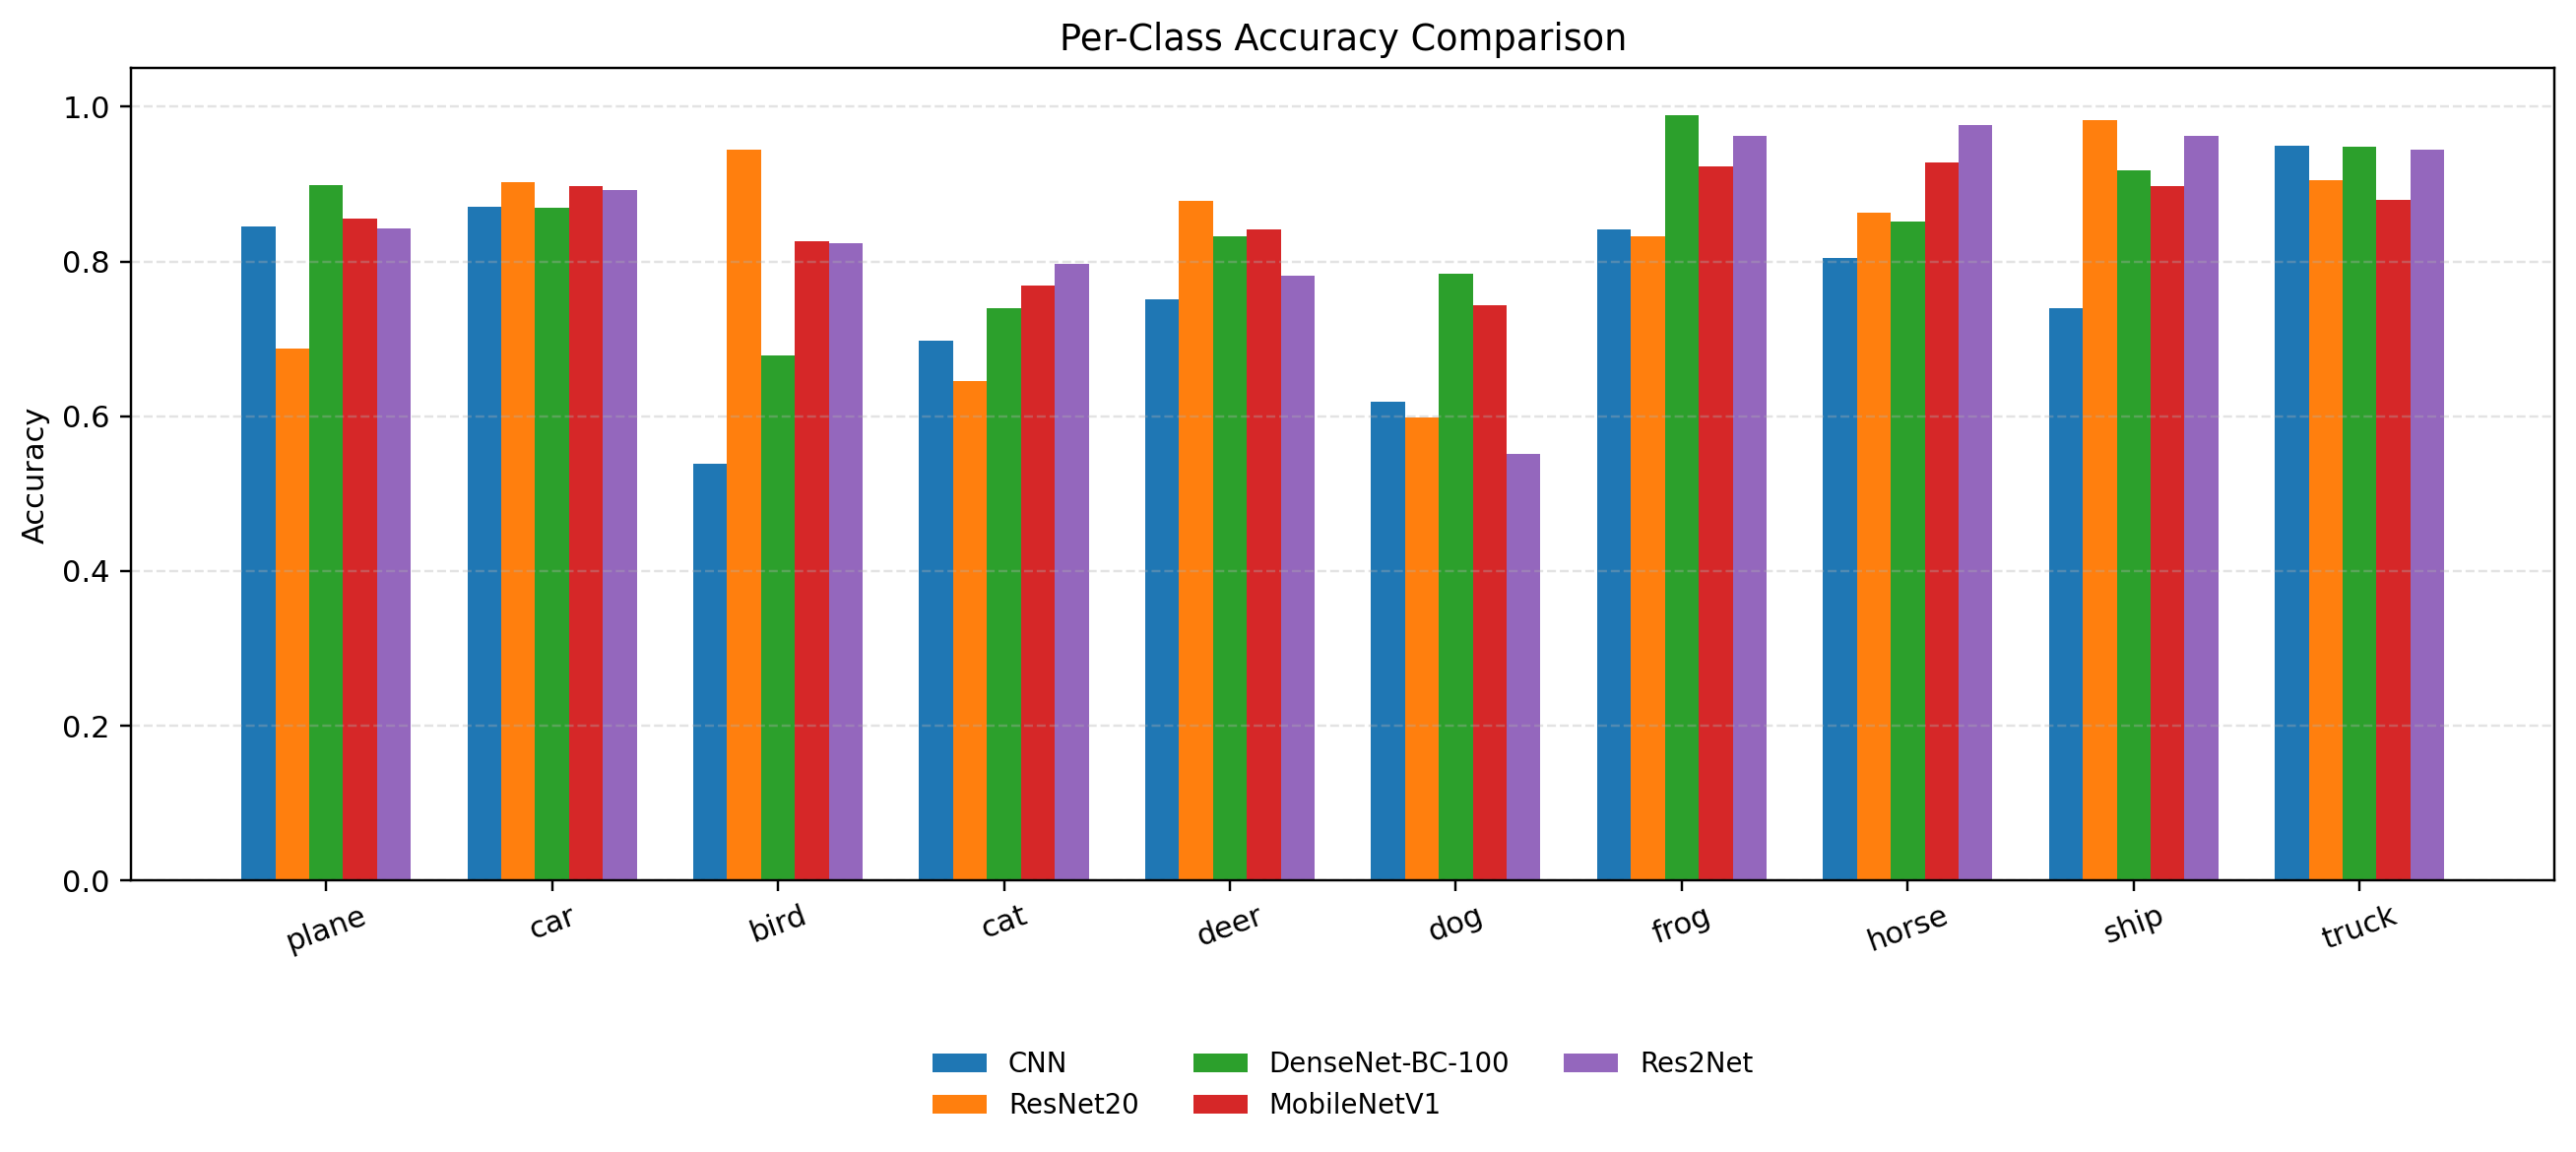
\includegraphics[width=\textwidth]{generated/class_accuracy.png}
    \caption{五种模型在最优学习率下的各类别准确率对比。}
\end{figure}

为了避免只通过总体准确率评价模型，本文进一步统计了各类别准确率。由于 CIFAR-10 测试集中各类别样本数相同，因此这里不再单独引入 BAcc 指标，否则其数值会与总体测试准确率高合，增加表格冗余而不会提供额外信息。

从各类别准确率分布可以看出，不同模型在 CIFAR-10 各类别上的表现并不均衡。多个模型在 \texttt{frog}、\texttt{ship}、\texttt{truck} 等类别上准确率较高，而在 \texttt{cat}、\texttt{dog} 等细粒度区分类别上更容易出现性能下降，说明这些类别之间的视觉相似性更强、判别难度更大。Res2Net、MobileNetV1 和 DenseNet-BC-100 在大多数类别上都保持了较高准确率，而原始 CNN 在多个类别上的识别能力都明显偏弱。因此，类别准确率分析能够补充说明不同网络在总体准确率之外的类别偏好与识别稳定性差异。

\subsection{不同卷积网络训练过程差异分析}
由于本实验采用的 batch size 为 512，相对较大，单个 epoch 内梯度估计的随机性被明显降低，因此多数模型的 train loss 和 train acc 曲线都较为平滑；但这并不意味着模型在泛化上同样稳定。相比之下，验证集曲线更容易出现波动，除了与学习率选择有关之外，还与以下因素有关：其一，验证集规模有限，统计量本身更敏感；其二，不同 epoch 的参数更新会首先反映在未见样本的预测置信度变化上，因此 val loss 往往比 val acc 更容易抖动；其三，部分模型参数量更大或结构更复杂，在训练后期更容易出现轻微过拟合，使得 train 曲线继续平稳改善，而 val 曲线开始震荡。因而，将 train 与 val 结合起来观察，能够更全面地区分“优化是否顺利”和“泛化是否稳定”这两个层面的差异。
\begin{enumerate}
    \item \textbf{原始 CNN：}
    原始 CNN 没有显式的跨层连接，特征只能沿网络深度逐层传递，因此当网络加深时，容易出现优化困难与表示能力不足的问题。从实验结果来看，CNN 的测试集准确率仅为 76.58\%，明显低于其余几种改进结构；同时虽然其参数量最小，仅有 111,050，FLOPs 也最低，但这说明其轻量化更多是以牺牲表征能力为代价换来的。从训练曲线看，CNN 的 train loss 虽然能够逐渐下降，但 val acc 提升较慢，最终上限也明显较低，说明其在 CIFAR-10 上的特征提取能力有限。换句话说，原始 CNN 可以作为最基础的卷积分类器，但在更复杂的图像识别任务中，其性能瓶颈较早出现。

    \item \textbf{ResNet：}
    ResNet 的核心思想是引入残差连接，使网络不必直接学习完整映射，而是学习相对于恒等映射的残差，从而缓解深层网络中的退化问题\cite{resnet}。实验结果表明，ResNet20 的测试集准确率达到 82.40\%，相比原始 CNN 提升明显，而参数量仅为 272,474，仍然保持在较低水平。从训练曲线看，ResNet 的 train loss 和 val loss 下降更加稳定，val acc 提升速度也更快，说明残差连接确实改善了优化过程，使梯度能够更顺畅地传播到浅层。结合效率指标来看，ResNet20 的 FLOPs 为 41,403,072，训练时间为 781.3 s，虽然比原始 CNN 更重，但其精度提升是明显值得的。因此，ResNet 体现出较好的“性能-复杂度”平衡，是一种结构较稳健、训练较可靠的深层卷积网络。

    \item \textbf{DenseNet：}
    DenseNet 进一步加强了跨层信息流动，它不是只连接相邻层，而是让每一层都直接接收前面所有层的输出，从而实现更充分的特征复用\cite{densenet}。实验中，DenseNet-BC-100 的测试集准确率为 85.13\%，高于 ResNet20，说明密集连接确实增强了特征表达能力。从训练曲线看，DenseNet 的 val acc 上升较快，最终验证集最佳准确率也较高，反映出其较强的特征传播与复用能力。然而，这种结构的代价也很明显：由于每层输出都要拼接到后续层中，通道数会不断累积，因此训练时间显著增长，达到 2921.7 s，FLOPs 也达到 300,797,106，明显高于 ResNet20 和 MobileNet。也就是说，DenseNet 在精度方面具有优势，但其局限在于显存与计算开销更大，实现与训练成本更高。

    \item \textbf{MobileNet：}
    MobileNet 的重点并不是单纯提升精度，而是在准确率和效率之间取得更好的折中。它通过深度可分离卷积，将标准卷积分解为 depthwise convolution 和 pointwise convolution，从而显著降低计算量\cite{mobilenet}。在实验中，MobileNetV1 的测试集准确率为 85.64\%，是几种基础改进网络中最高的，同时 FLOPs 仅为 41,195,008，与 ResNet20 接近，推理时间也较短，说明其在轻量化设计上具有明显优势。从训练曲线看，MobileNet 的收敛过程整体较平稳，val acc 也能达到较高水平，说明这种卷积分解方式在保持效率的同时，并未严重破坏模型的表达能力。不过，它的参数量达到 1,618,250，高于 ResNet20，这说明 MobileNet 的优势主要体现在降低计算量，而不一定体现在参数量绝对最小。因此，MobileNet 更适合强调推理效率和部署成本的应用场景。

    \item \textbf{Res2Net：}
    Res2Net 在残差结构内部进一步引入多尺度特征表示，通过在单个残差块中划分多个尺度分支并逐级融合，使模型能够在更细粒度上建模不同感受野的信息\cite{Res2Net}。从实验结果看，Res2Net 的验证集最佳准确率达到 89.52\%，在所有模型中最高，测试集准确率为 85.34\%，也保持在较高水平，说明其多尺度建模确实增强了特征表达能力。从训练曲线来看，Res2Net 的 val acc 提升较快，并且能够达到较高平台，说明模型在训练过程中具有较强的拟合和表征能力。但其代价同样非常明显：参数量达到 3,461,834，FLOPs 高达 913,271,808，总训练时间为 3389.6 s，是几种模型中资源消耗最大的。这表明 Res2Net 的优势主要体现在更强的多尺度表达能力，而其局限在于模型更复杂、计算与显存开销更高。在 CIFAR-10 这类规模相对有限的数据集上，Res2Net 虽然能够取得更高验证性能，但其额外资源代价也需要综合考虑。
\end{enumerate}

\subsection{学习率敏感性与泛化稳定性补充分析}
\begin{table}[htbp]
\centering
\caption{Learning-rate sensitivity and generalization stability}
\scriptsize
\begin{tabular}{lcccc}
\toprule
Model & Val Acc Range & Best LR Gap & Final Acc Gap & Val Loss Rebound \\
\midrule
CNN & 0.1962 & 0.0014 & 0.044 & 0.124 \\
ResNet20 & 0.0492 & 0.0086 & 0.108 & 0.190 \\
DenseNet-BC-100 & 0.1268 & 0.0036 & 0.063 & 0.058 \\
MobileNetV1 & 0.0532 & 0.0196 & 0.095 & 0.070 \\
Res2Net & 0.0584 & 0.0090 & 0.110 & 0.185 \\
\bottomrule
\end{tabular}
\label{tab:sensitivity_stability}
\end{table}

\paragraph{学习率敏感性}
从表 \ref{tab:sensitivity_stability} 可以看出，不同模型对学习率的敏感程度存在明显差异。若以 6 个学习率下的最佳验证准确率波动范围衡量，原始 CNN 的波动最大，达到 0.1962；DenseNet-BC-100 次之，为 0.1268；而 ResNet20、MobileNetV1 和 Res2Net 的波动范围分别为 0.0492、0.0532 和 0.0584，整体更稳定。这说明原始 CNN 和 DenseNet 对学习率更敏感，而 ResNet20、MobileNetV1 与 Res2Net 在本实验设置下具有更好的超参数鲁棒性。进一步看最优点附近的差异，Res2Net 的最佳学习率为 0.05，对应的最佳验证准确率为 89.52\%，次优学习率 0.1 时为 88.62\%，二者相差 0.90 个百分点，说明其高性能仍依赖合适的学习率，但并未表现出极端难调的特征。

\paragraph{泛化稳定性}
从最优学习率对应的训练过程看，train 曲线整体较平滑，而 val 曲线更能体现泛化稳定性。若以最终的 train-val accuracy gap 衡量，CNN、DenseNet-BC-100、MobileNetV1、ResNet20 和 Res2Net 分别约为 0.044、0.063、0.095、0.108 和 0.110。由于 CNN 本身拟合能力较弱，其 gap 最小并不代表泛化最好；在高性能模型中，DenseNet 的 gap 相对较小，而 ResNet20 与 Res2Net 的 gap 更大，说明后两者在训练后期更容易出现“训练继续改善而验证收益有限”的现象。若进一步看 val loss 相对其最小值的回升幅度，DenseNet-BC-100 和 MobileNetV1 分别仅回升约 0.058 和 0.070，而 ResNet20 与 Res2Net 分别回升约 0.190 和 0.185，说明后两者在后期验证损失上的波动更明显。综合来看，Res2Net 虽然取得了最高的最佳验证准确率，但其泛化稳定性并不是最优，这也说明高表达能力模型通常伴随着更高的训练后期波动与更明显的过拟合风险。

\subsection{Res2Net 与其他网络的优缺点分析}
\paragraph{Insight}
Res2Net 论文的核心观点是：传统 ResNet 更强调“跨层残差连接”，但单个残差块内部的尺度表达仍然相对单一，因此作者提出在一个残差块内部再进行多尺度划分与逐级融合，从而在不显著增加网络深度的前提下增强特征的多尺度表示能力\cite{Res2Net}。从这个角度看，Res2Net 相比原始 CNN 和 ResNet 的主要优势在于：它不只是改善梯度传播，而是进一步提升了单个 block 内部的感受野层次，因此对于不同尺度目标或复杂纹理模式通常具有更强的表达能力。本实验中，Res2Net 取得了最高的最佳验证准确率，也说明这种多尺度建模思路在 CIFAR-10 上具有实际效果。

\paragraph{与 ResNet 的比较}
相较于 ResNet，ResNet 的优点在于结构更简洁、训练更稳定、参数量和计算量都更容易控制\cite{resnet}；而 Res2Net 则是在 ResNet 残差框架基础上进一步增强 block 内部的多尺度表示，因此通常能获得更强的特征表达能力，但代价是结构更复杂、显存和计算开销显著增加。从本实验结果看，Res2Net 的精度上限略高于 ResNet20，但其 FLOPs 和训练时间都远高于后者，因此二者更适合不同场景：若追求稳健和高性价比，ResNet 更合适；若更关注表示能力和精度上限，Res2Net 更有优势。

\paragraph{与 DenseNet 的比较}
DenseNet 提供的是另一种提升性能的路径。其论文强调特征复用与信息流加强，即通过密集连接让后续层直接访问前面所有层的输出\cite{densenet}。DenseNet 的长处在于参数利用率高、特征传递充分，而 Res2Net 的重点并不在跨层复用，而是在单个 block 内构造更细粒度的尺度层次。因此，两者提升性能的路径并不相同：DenseNet 更像是“加强跨层连接”，Res2Net 更像是“加强块内多尺度表示”。从实验现象看，DenseNet-BC-100 与 Res2Net 都取得了较高精度，但 DenseNet 已经具有较大的训练时间开销，而 Res2Net 还进一步增加了计算复杂度，说明后者虽然表征能力更强，但代价也更高。

\paragraph{与 MobileNet 的比较}
从设计目标上看，MobileNet 与 Res2Net 的差异最明显。MobileNet 的设计目标是以较低计算成本获得可接受精度，其论文强调的是 depthwise separable convolution 带来的效率优势\cite{mobilenet}。因此 MobileNet 代表的是“效率优先”的设计思想，而 Res2Net 代表的是“表达能力优先”的设计思想。本实验中，MobileNetV1 的测试准确率已经相当有竞争力，同时 FLOPs 和推理时间明显优于 Res2Net，这说明在资源受限或部署场景下，MobileNet 更实用；而 Res2Net 则更适合对特征表达要求更高、对资源约束相对宽松的场景。

\paragraph{综合评价}
综合来看，Res2Net 的主要优点在于：能够在保持残差框架优点的同时增强多尺度特征建模能力，因而在验证集性能和整体类别平均识别能力上都较强；其主要缺点在于：结构复杂度、参数量、FLOPs、训练时间和显存占用都更高。对于本实验所使用的 CIFAR-10 小尺寸数据集而言，Res2Net 的性能提升是真实存在的，但其额外资源代价也非常明显，因此它更适合作为“高表达能力模型”的扩展对照，而不是所有场景下都最优的默认选择。

\subsection{类激活映射可视化分析}
\begin{figure}[htbp]
    \centering
    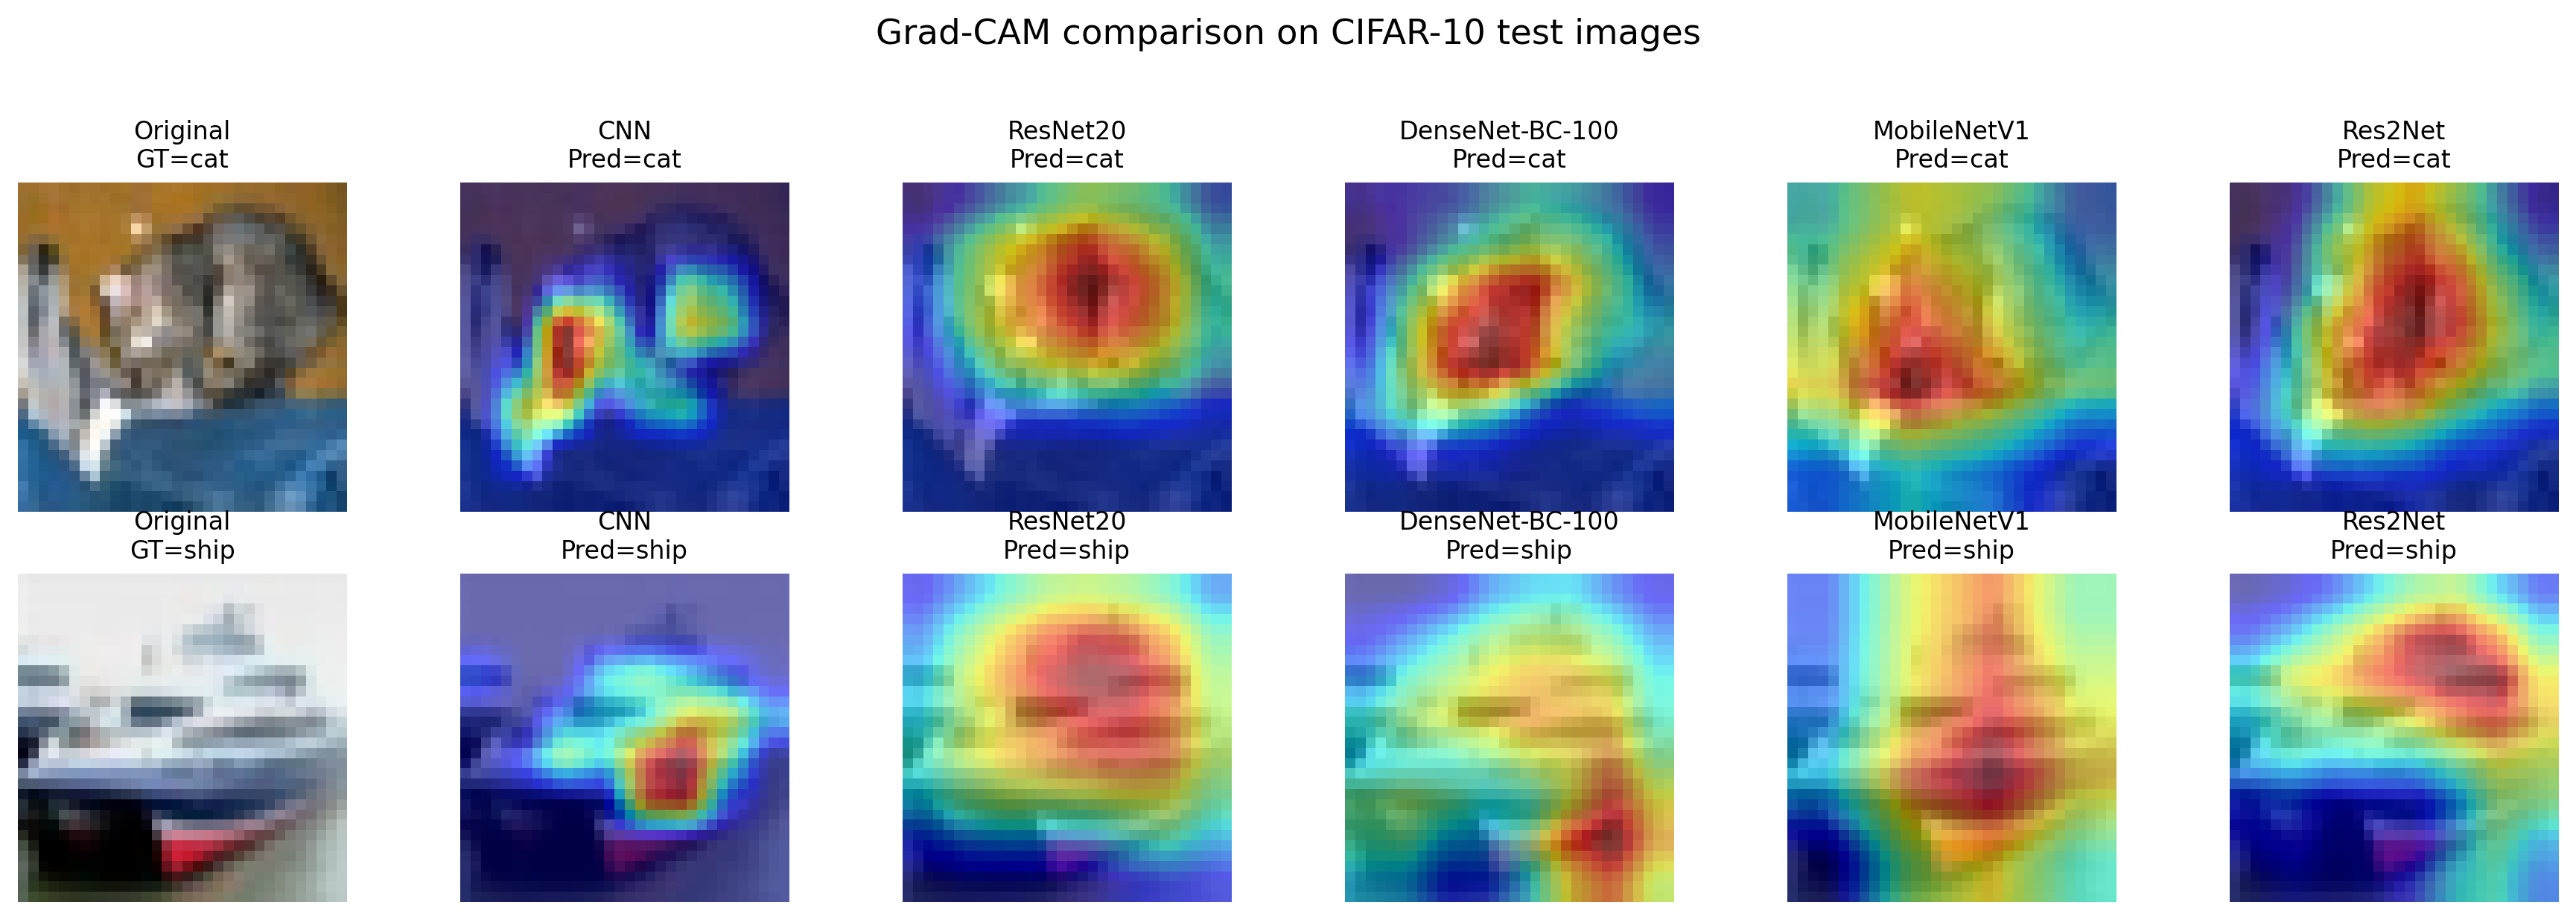
\includegraphics[width=\textwidth]{generated/gradcam_comparison.png}
    \caption{五种模型在 CIFAR-10 测试样本上的 Grad-CAM 可视化对比。每行对应一张测试图像，第一列为原图，后续各列为不同模型对预测类别的响应热力图。}
\end{figure}

为了进一步观察不同模型的判别依据，本文采用 Grad-CAM 对五种模型进行可视化分析。整体来看，原始 CNN 的激活区域通常更局部，容易集中在目标的某一小块纹理上；ResNet20 的响应区域相对更稳定，但仍偏向于目标的主要判别部位；DenseNet-BC-100 与 MobileNetV1 的关注区域往往更加完整，其中 DenseNet 更容易覆盖较大范围的目标结构，而 MobileNet 的响应则相对集中。相比之下，Res2Net 的热力图通常在目标主体上形成更连续的高响应区域，这与其块内多尺度特征建模能力是一致的，也从可视化角度支持了其较高的验证性能。当然，这种更强的响应能力仍然伴随着更高的计算和训练代价，因此可视化结果进一步说明，Res2Net 的优势主要体现在表达能力，而劣势则体现在效率成本。

\section{实验结论}
本实验完成了原始 CNN、ResNet20、DenseNet-BC-100、MobileNetV1 以及扩展模型 Res2Net 的实现与比较。实验结果表明，带有跳跃连接或密集连接的网络在 CIFAR-10 上明显优于普通卷积网络。ResNet20 结构稳定、参数量适中；DenseNet-BC-100 具备较强的特征复用能力；MobileNetV1 在轻量化方面优势明显；Res2Net 在多尺度特征提取方面具有潜力，但计算代价也更高。总体而言，不同模型在精度、效率与训练稳定性之间体现出了不同的权衡关系。

\appendix
\section{代码目录说明}
为便于查阅与提交，本实验将所有代码统一整理在 \texttt{lab1/code/} 目录下，而数据、实验结果和报告分别保留在根目录中的 \texttt{data/}、\texttt{outputs/} 和 \texttt{实验模板/} 中。教师若希望快速定位核心代码，建议优先查看以下文件：

\begin{itemize}
    \item \texttt{code/train.py}：单次训练入口；
    \item \texttt{code/sweep\_lr.py}：学习率扫描入口；
    \item \texttt{code/src/models/}：各模型实现，包括 \texttt{simple\_cnn.py}、\texttt{resnet.py}、\texttt{densenet.py}、\texttt{mobilenet.py} 和 \texttt{res2net.py}；
    \item \texttt{code/src/engine.py}：训练、验证、测试主循环；
    \item \texttt{code/src/data.py}：CIFAR-10 数据加载与划分；
    \item \texttt{code/scripts/generate\_report\_assets.py}：报告曲线图与表格生成；
    \item \texttt{code/scripts/generate\_gradcam\_report.py}：Grad-CAM 可视化生成。
\end{itemize}

\noindent 当前代码目录结构如下：
\begin{verbatim}
code/
|-- train.py
|-- sweep_lr.py
|-- src/
|   |-- config.py
|   |-- constants.py
|   |-- data.py
|   |-- engine.py
|   |-- models/
|   `-- utils/
|-- scripts/
`-- legacy/
\end{verbatim}

\newpage
\bibliographystyle{plain}
\bibliography{reference}

\end{document}
